\documentclass[a4paper,12pt]{report}
\usepackage[utf8]{inputenc}
\usepackage[T1]{fontenc}
\usepackage{lmodern}
\usepackage{mathtools}
\usepackage[catalan]{babel}
\usepackage{hyperref}
\usepackage{graphicx}
\usepackage{acronym}
\usepackage{eurosym}
\usepackage{pgfplots}
\usepackage[auth-sc]{authblk}
\date{}
\begin{document}

% Arxiu per als acrònims
\acrodef{foss}[FOSS]{Free Open Source Software}
\acrodef{fsf}[FSF]{Free Software Foundation}


\title{
	{\bf Filosofia del Software i Intel·ligència Artificial}
}
\author{
	Oriol Ventosa \and
	Marc Ferré \and
	Gonzalo Palacios \and
	Pol Gómez
}

\maketitle

\tableofcontents

\chapter{Introducció}
Aquest projecte de recerca es divideix en dues parts; els \emph{conceptes}
i els \emph{procediments}.

El \emph{software}, les seves filosofies i llicències formaran el primer i més
teòric apartat. S'explicarà què és el software i es separarà en \emph{propietari}
i \emph{lliure}, dues formes de veure la creació i distribució del mateix. A més,
s'introduirà la \emph{intel·ligència artificial} (IA), la seva història, el seu present i el
seu hipotètic futur, com a preludi pels procediments del projecte.

En la segona part, sobre \emph{intel·ligència artificial}, s'explicarà el procés
que s'ha seguit per a crear un seguit de \emph{demostracions}, que apliquen un
dels mètodes més coneguts de la IA; les \emph{xarxes neuronals}. A través de demostracions
gràfiques es podrà entendre millor en concepte de les ANN (\emph{Artificial Neural Networks}).

Amb aquest projecte es pretén trobar un punt en comú entre les matemàtiques,
la intel·ligència artificial i el software (específicament, lliure), a més de
respondre a una pregunta que molts ens haurem fet en algun moment: \emph{és possible crear
intel·ligència artificial?}

S'ha treballat de forma altament col·laborativa, a través d'una plataforma
en línia anomenada \href{http://github.com}{GitHub}, que implementant un sistema
de control de versions anomenat \href{http://git-scm.com/}{Git}, descentralitza
el projecte, i permet el lliure accés a col·laboradors externs i, especialment, a membres
del mateix grup. Permet mantenir en sincronització el projecte i fusionar canvis entre els integrants del grup.

Per a realitzar l'escrit, s'ha utilitzat \LaTeX, un llenguatge de programació que permet escriure documents de forma molt més flexible, multiplataforma i lleugera, a més de facilitar la col·laboració entre diferents persones. També introdueix una forma d'escriure la bibliografia molt més pragmàtica i viable, que actualitza les referències sense haver de fer-ho manualment, i crea l'índex automàticament.


\chapter{El Software}
\section{Què és?}
El \emph{software} o \emph{programari} és el conjunt dels programes informàtics, procediments i documentació que fan alguna tasca en un ordinador. Per tant, qualsevol eina que s'executa en el nostre ordinador, que té una tasca definida, es pot definir com a programari. Casualment, la major part d'eines que executem diàriament en els nostres ordinadors, duen a terme alguna tasca
(navegar internet, crear un document, consultar el correu electrònic, etc). Per tant, un ordinador sense programari, serveix de ben poc.

\emph{Paint}, \emph{Photoshop}, \emph{GIMP}, \emph{Steam}, \emph{Firefox}, \emph{Dropbox}, \emph{Office}, \emph{Avast}... tots aquests noms fan referència a programes, software. És 
sense dubte complicat imaginar un ordinador sense cap d'aquests elements instal·lats, veritat?

\section{Com es crea?}
El programari, encara que sembli redundant, es programa. Els \emph{programadors}
són enginyers que desenvolupen aquest programari. Per a crear software, s'utilitzen
\emph{llenguatges de programació}, que n'hi han molts (\emph{C, Python, Lisp, Haskell...})
i cadascun amb el seu propòsit diferent. Quan s'ha completat el disseny d'un programa
(es a dir, s'ha programat el \emph{codi font} \footnote{Instruccións que se li donen al
llenguatge de programació}), aquest es \emph{compila} a \emph{codi de màquina} \footnote{Text indesxifrable per al cervell humà, però que els sistemes operatius entenen}, que l'ordinador llegeix i executa.

Si es detecta un mal funcionament en algun moment en l'execució del programa, anomenat \emph{bug}, els
programadors revisen el codi font, fan les correccions necessàries, compilen el programa,
i el distribueixen altre cop.

Quan l'usuari adquireix el programari en format de codi de màquina, o \emph{binari}, només el pot
executar. És molt complicat desxifrar el codi original a partir del producte final, però és una
pràctica que solen realitzar les comunitats de \emph{crackers}, i s'anomena \emph{enginyeria inversa}.

Però no només els desenvolupadors de programari són qui compilen el codi font; depenent de la forma
de distribució del software, l'usuari final pot compilar el software, i fins i tot, fer-hi modificacions. Però, que l'usuari tingui aquesta oportunitat o no,  dependrà de si el software que ha adquirit es regeix per una llicència \emph{lliure} o \emph{propietària}.

\begin{figure}[ht!]
\centering
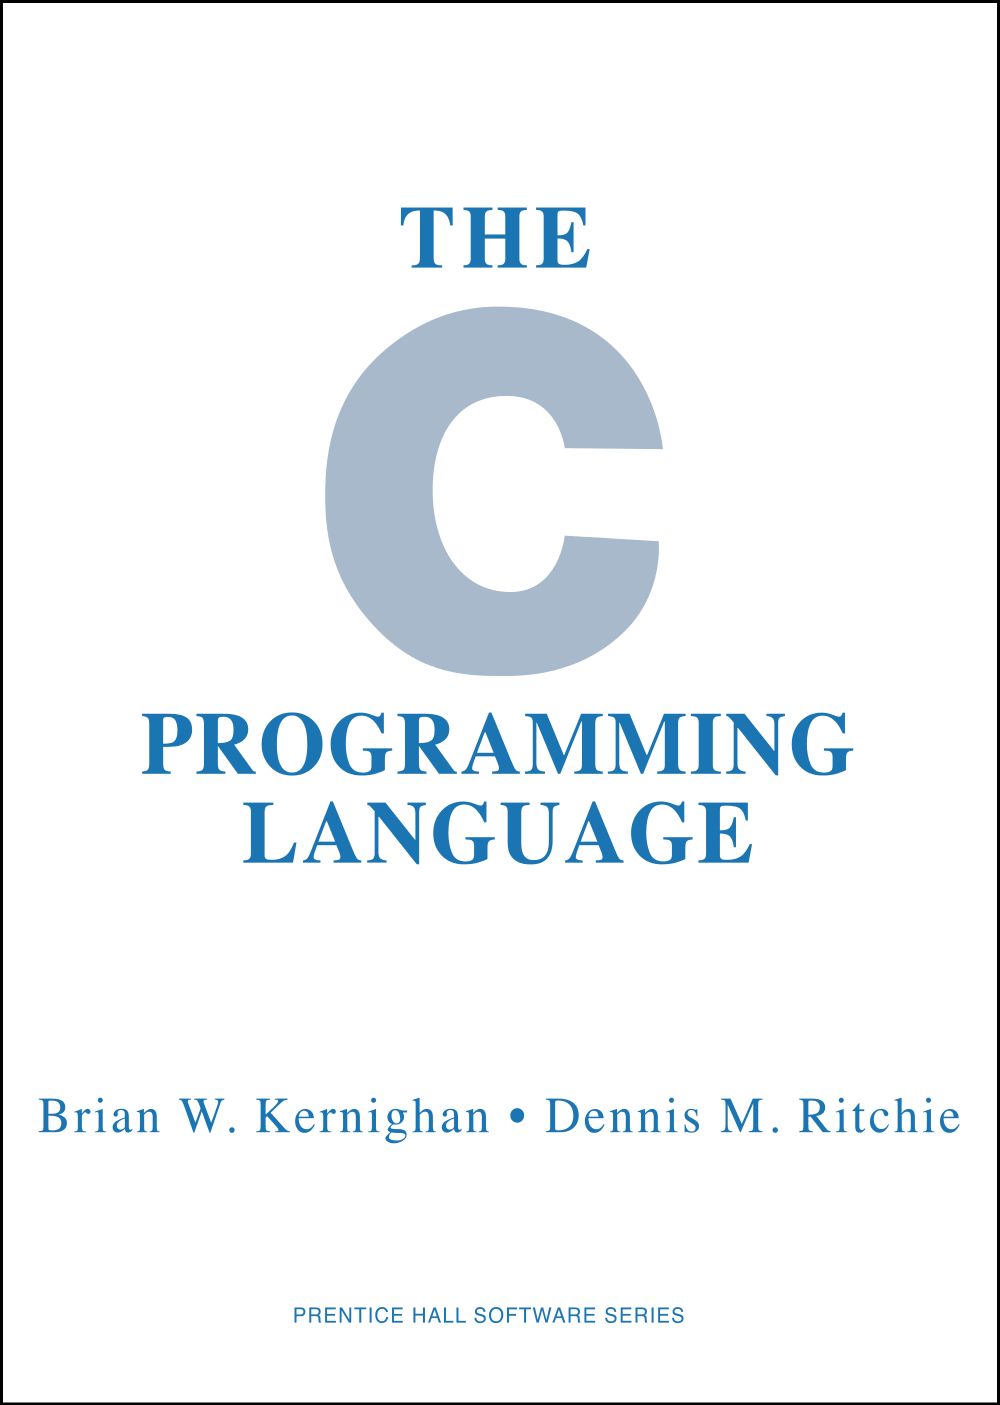
\includegraphics[height=75mm]{data/clang.png}
\caption{Portada del llegendari llibre que explica programació amb el llenguatge \emph{C}, de \emph{Kernighan} i \emph{Ritchie}, els dos desenvolupadors principals.}
\label{websshare}
\end{figure}


\chapter{El Software Lliure}
\section{Què és?}

El software lliure (de l'anglès \emph{"free software"}) és tot aquell software publicat
sota llicències que respecten el concepte de \emph{llibertat}. Degut a que la definició
(en relació al software) de llibertat és molt àmplia, i es podria dedicar inacabable espai
a definir-la, utilitzarem la definició més acceptada, la que ha popularitzat la \ac{fsf}; \emph{un programa és lliure si al adquirir-lo, l'usuari pot fer-lo servir,
copiar-lo, estudiar-lo, modificar-lo, i redistribuir-lo lliurement de diferents formes}. \cite{wikifree}

Que el software sigui lliure, no implica que el seu cost sigui zero (encara que molt
software lliure, també sigui gratuït) \cite{sellingfree}. Per tant, jo puc crear software lliure i distribuir els arxius
binaris a \EUR{500,000}, mentre mantingui un lliure accés al codi font. El desenvolupament de software
lliure es sol finançar a través de donacions voluntàries, i la major part de projectes dediquen
aquests diners recaptats al manteniment dels serveis que el software que distribueixen necessita
(cost dels servidors i manteniment web, etc).

\section{Qui el fa?}

La major part de software lliure no és realitzat per companyies multimilionàries; en canvi,
petits i mitjans grups de desenvolupadors són qui donen vida a la gran comunitat de software lliure.
Tot i això, la major part de projectes de software lliure relativament importants
són suportats i actualitzats per empreses que no es dediquen exclusivament a \emph{crear}
software lliure, però que n'utilitzen, i això les motiva a millorar-lo (per exemple, \emph{HP, IBM, Intel, Oracle, Samsung, AMD, Google, Cisco, Toyota, Panasonic, Adobe, Dell, Epson, LG, Nokia, Nissan, Nvidia, Sony, Siemens, Toshiba, Yahoo...}\cite{linuxmembers}).

Definir la importància del software lliure basat en el nombre d'empreses que hi col·laboren no és la forma més correcta de fer-ho; hi han milers de programadors que actualitzen programari lliure cada dia, molts d'ells de forma altruista, i això no incrementa el nombre d'empreses.

La comunitat de software lliure és extremadament viva, i omple tots els tipus de programari que un usuari pugui desitjar. Per exemple; el projecte \emph{Linux} accepta setmanalment un mitja de 750 col·laboracions en el seu codi font, i té més de 3,500 col·laboradors actius \cite{linuxgitrepo}. El reproductor de vídeo i audio \emph{VLC} (un projecte més petit, que Linux, evidentment), té una mitja de 200 col·laboracions setmanals \cite{vlcgitrepo}. Dia a dia, desenvolupadors individuals o grups reduïts utilitzen diferents plataformes a internet per a iniciar els seus projectes de software lliure, i permetre la col·laboració amb molts més programadors.

\section{Història}

Des dels anys 50 fins als 70, no hi havien grans corporacions que 
llicenciessin software, i es solia compartir de forma lliure entre
programadors, i distribuir de forma integrada en el \emph{hardware}
(es a dir, els ordinadors). Una vegada entrats en els 70, la indústria del
software va començar a mostrar la seva capacitat econòmica, i es va
començar a vendre programari per separat. \cite{ibmusdata}

En \emph{Richard Matthew Stallman}, va anunciar el projecte \emph{GNU} (\emph{GNU no és Unix!}, conjunt d'utilitats per a iniciar un sistema operatiu lliure), argumentant que s'havia cansat dels efectes del canvi en la cultura de la indústria informàtica i els seus usuaris. La FSF (\emph{Free Software Foundation}) va ser fundada l'Octubre de 1984, i va desenvolupar una de les definicions de \emph{software lliure} més acceptades, i el concepte de \emph{copyleft}, dissenyat per a assegurar la llibertat de software per a tothom. \cite{fossieee}.

A partir d'aquell moment, la comunitat de software lliure va començar a créixer.

\begin{figure}[ht!]
\centering

\includegraphics[width=100mm]{data/fsf.png}
\caption{El logotip de la \ac{fsf}.}
\label{fsfpic}
\end{figure}

\section{Us actual}

En l'actualitat, hi ha molt software lliure en circulació activa, i una gran comunitat de desenvolupadors darrere d'ell, però no és tant popular com el software propietari (que no vol dir que no sigui utilitzat tant).

No només els usuaris particulars tenen a l'abast (i utilitzen) software lliure: molts governs han fet (o estan fent) el traspàs al software d'aquest tipus (Kerala, a la Índia, Munich, a Alemanya, Veneçuela, Malàisia, Perú, Equador, i altres). \cite{fossadopters}

\section{Avantatges i inconvenients}

El software lliure té una quantitat important d'avantatges  \cite{fossadvantages}:

\begin{enumerate}
\item \emph{Econòmic} - molta part del FOSS (software de codi obert i lliure) és gratuït, o té un preu molt baix. Les petites empreses es poden beneficiar d'això, i expandir la seva infraestructura informàtica sense gastar milers d'euros en software propietari.
\item \emph{Llibertat d'ús i distribució} - es pot instal·lar software lliure sense limitacions per culpa de llicències d'un sol ús, com passa amb els sistemes operatius i 'suites' ofimàtiques.
\item \emph{Independència tecnològica} - l'accés al codi font permet desenvolupar nous productes amb una base sòlida de software, o ajustar-lo a les nostres necessitats. Quan s'utilitza software lliure, no s'ha de patir per les decisions de l'entitat creadora, ja que sempre es tindrà accés a versions més antigues, o en casos més avançats, al codi font.
\item \emph{Sistemes sense 'backdoors'} - tenir accés al codi impossibilita la implementació de \emph{espies} en el codi font d'un programa.
\item \emph{Correcció més ràpida i eficient d'errors} - la comunitat activa de desenvolupadors de software lliure realitzen actualitzacions constants, i errors o 'bugs' són arreglats molt més ràpid que en el software propietari.
\end{enumerate}

De totes formes, també té desavantatges \cite{gentegeek}:

\begin{enumerate}
\item \emph{Falta de garantia} - el software lliure no ofereix garanties; si es trenca, no és culpa de ningú excepte teva, si es que has fet alguna cosa malament.
\item \emph{Difícil d'adquirir} - hi ha una certa quantitat de software lliure que és més complicat de descarregar i instal·lar en comparació amb el seu germà propietari. Es deu, en molts casos, en que els autors es centren en el \emph{codi} del programa, i no tenen els recursos suficients per assegurar la disponibilitat de paquets compilats per a cada plataforma.
\item \emph{Acabat final} - molt software lliure ofereix un aspecte gràfic o final poc atractiu; no hi han equips dedicats íntegrament al desenvolupament de l'interfície gràfica, i es fa el que es pot, amb els recursos que es tenen.
\item \emph{Entreteniment} - els títols \emph{AAA} (jocs amb pressupost molt elevat) no són lliures. Falta molt de temps per a que l'usuari comú pugui observar l'impressionant codi font de títols com \emph{Battlefield} o \emph{Far Cry}, ja que el mercat és més lucratiu que ètic, i s'hi troben molts inconvenients en alliberar el codi font d'un \emph{engine} (motor gràfic).
\end{enumerate}

\begin{figure}[ht!]
\centering
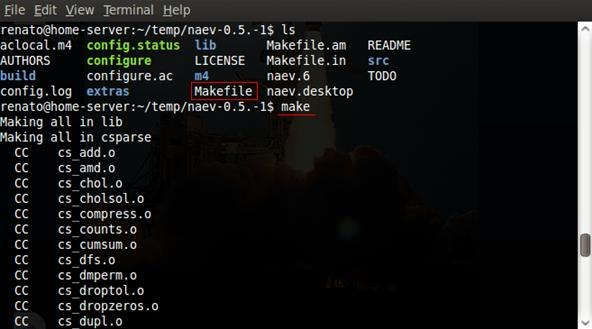
\includegraphics[width=100mm]{data/linuxcompile.jpg}
\caption{Procés de compilació de Linux (\href{http://renatonel.wonderhowto.com/inspiration/first-steps-compiling-program-linux-0127658/}{wonderhowto.com}).}
\label{websshare}
\end{figure}

\chapter{El Software Propietari}
\section{Què és?}

	Anomenem software propietari a tot aquell programa publicat sota llicències
	que reserven un o tots els drets d'ús, còpia, modificació i distribució
	al fa- bricant qui, pagant, concedeix un ús del programa executable al titular
	de la llicència.

	Per tant, el software \emph{propietari} o \emph{privatiu} obstrueix la llibertat
	de l'usuari final, que quan ha adquirit el programa, té uns drets limitats i fortes
	obligacions, que solen incloure la impossibilitat d'adquirir i modificar el codi font del producte
	que ell mateix ha comprat, tant com la prohibició total o parcial de la redistribució del programa.
	\cite{gnucategories}

	Per a entendre millor el software propietari, posem un exemple pràctic:	en Jaume crea un programa impressionant, amb l'ajut de diferents col·laboradors (que ho fan com a hobby),
	i distribueix el programa a través d'una llicència permissiva (per exemple, la BSD). Amb el temps, més gent col·labora i cada vegada,
	aquest programa fet amb l'esforç de centenars de voluntaris, adquireix més importància en el món del \emph{software}.
	En Jaume, però, segueix volent mantenir la filosofia lliure del software que la comunitat ha creat, i per tant
	manté la llicència permissiva.
	
	Un dia, una companyia, agafa tot el codi d'en Jaume, el modifica lleuge- rament, i
	el redistribueix amb una llicència propietària. Ara, totes les millores que es podrien haver incorporat
	al codi d'en Jaume a benefici de la comunitat, estan en mans d'una gran corporació, que no les vol compartir.
	Degut a la llicència que en Jaume ha fet servir, no té dret a res, i la comunitat que ha treballat durant tot aquest temps,
	es quedarà sense les millores que la corporació ha desenvolupat, sobre la seva base.
	
	Aquesta situació es pot evitar o repetir, tot depèn de la llicència que en Jaume esculli al crear el seu següent programa.

\section{Qui el fa?}

	El principal desenvolupador de software propietari a nivell mundial és \emph{Microsoft}, encara que hi
	ha moltes més empreses que també en creen i distribueixen, com \emph{Apple, Oracle, Adobe, VMware,
	SAP, Symantec...} \cite{propietariempreses}

\section{Ús actual}

	Avui en dia molta part del software utilitzat per la majoria de població, és propietari.

	Aquesta gran extensió del seu ús és degut a l'inversió milionària al màrketing, i a
	pactes amb productors de sistemes operatius i proveïdors d'Internet, que acorden la
	prèvia instal·lació de software propietari als ordinadors. Junt amb la falta d'informació del que 
	comporta l'ús de programes propietaris, i la falta de preocupació de la integritat dels
	nostres drets virtuals, son els motius principals de l'expansió del software propietari.

	\begin{figure}[ht!]
	\centering
	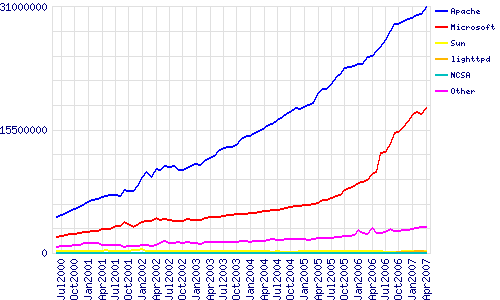
\includegraphics[width=100mm]{data/web_servers_share.png}
	\caption{Ús de software en servidors web \cite{whyfoss}}
	\label{websshare}
	\end{figure}

	\begin{figure}[h!]
	\centering
	\begin{tikzpicture}
	\begin{axis}[
		ybar,
		enlargelimits=0.15,
		legend style={at={(0.5,-0.2)},
		anchor=north,legend columns=-1},
		ylabel={\% Ús de sistemes operatius (2013)},
		symbolic x coords={Windows,MacOS,GNU/Linux,Mòbil},
		xtick=data,
		nodes near coords,
		nodes near coords align={vertical},
		x tick label style={rotate=45,anchor=east},
	]
	\addplot coordinates {(Windows,82.57) (MacOS,9.55)
	(GNU/Linux,4.85) (Mòbil,2.72)};
	\end{axis}
	\end{tikzpicture}
	\caption{Ús de sistemes operatius per a particulars \cite{osstats}}
	\label{osshare}
	\end{figure}

	\begin{figure}[h!]
	\centering
	\begin{tikzpicture}
	\begin{axis}[
		ybar,
		enlargelimits=0.15,
		legend style={at={(0.5,-0.2)},
		anchor=north,legend columns=-1},
		ylabel={\% Ús de sistemes operatius (2013)},
		symbolic x coords={Windows,Unix,MacOS},
		xtick=data,
		nodes near coords,
		nodes near coords align={vertical},
		x tick label style={rotate=45,anchor=east},
	]
	\addplot coordinates {(Unix,66.8) (Windows,33.3) (MacOS,0.1)};
	\end{axis}
	\end{tikzpicture}
	\caption{Ús de sistemes operatius per a servidors \cite{ossvstats}}
	\label{ossvshare}
	\end{figure}

	El gràfic \ref{websshare} mostra la distribució (o \emph{market share}) de diferents companyies de software
	en l'àmbit dels servidors web
	\footnote{Ordinadors que funcionen el màxim de temps possible i comparteixen l'accés a una direcció web.
	Per exemple, \emph{Google} té molts servidors que permeten l'accés públic als seus serveis.}.
	\emph{Apache}\cite{apache} ha mantingut sempre la seva posició,
	seguit per \emph{Microsoft} i altres companyies. En aquest cas, el software lliure (de la mà de la
	llicència \emph{Apache 2.0}\cite{apachelicense}) és prevalent de llarg.

	El gràfic \ref{osshare} mostra el market share de \emph{sistemes operatius} que utilitzen els particulars
	(qualsevol persona). \emph{Microsoft Windows} és el guanyador indiscutible, amb \emph{MacOS} molt per darrere
	i els sistemes operatius \emph{GNU/Linux} (l'alternativa lliure) amb menys del 5\% del share.

	El gràfic \ref{ossvshare} mostra el market share de sistemes operatius que utilitzen els servidors i,
	al igual que en els programes que utilitzen els servidors, el software lliure guanya.
	
	D'aquests documents podem extreure una conclusió ben simple; la població general, no especialitzada,
	utilitza generalment software propietari (que, casualment, els hi ve pre-instal·lat als ordinadors).
	En canvi, els usuaris especialitzats (mantenidors de servidors, en aquest cas), es passen a les alternatives
	de software lliure, que amb el temps han demostrat més viabilitat i seguretat per al ús que s'els hi ha de donar.
	Per tant, el software propietari és majoritari per \emph{conveniència}, no per qualitat.


\section{Avantatges i inconvenients}

Els avantatges principals del software propietari  són ben simples; solen ser avantatges per part
de l'empresa creadora, ja que generen beneficis més elevats que el software lliure (que es sol distribuir
de forma gratuïta) \cite{gentegeek}.

Per part de l'usuari, en podem extreure alguns:

\begin{enumerate}
\item \emph{Atenció al client}: molt software lliure no ofereix ni garanties, ni atenció al client 'professional'.
La major part d'empreses de software propietari es veuen obligades a oferir-ne, ja que si no, el seu producte (generalment,
que comporta un cost econòmic) perd reputació i clientela.
\item \emph{Fàcil adquisició:} avantatge per a alguns, inconvenient per a uns altres (no volen software pre-instal·lat als seus
ordinadors).
\end{enumerate}

En quant a inconvenients, en podem trobar bastants:
\begin{enumerate}
\item \emph{Falta de suport multi-plataforma}: molt software privatiu es centra en les plataformes principals (Windows i MacOS),
i s'oblida de les minoritàries.
\item \emph{Impossibilitat de modificació}: un programa propietari té un error amb solució simple, i tu tens coneixements de
programació? Oblida't d'arreglar-ho, hauràs d'esperar a una actualització oficial.
\item \emph{Impossibilitat de còpia}: en molts casos, si vols instal·lar un mateix software a diferents ordinadors de la teva
propietat, hauràs de comprar la mateixa llicència vàries vegades.
\item \emph{Falta de seguretat personal}: no pots saber si el software recull dades del teu ordinador, ni a qui les comparteix.
\item \emph{Dependència a l'empresa}: quan compres un programa, quedes subjugat a les decisions que l'empresa faci sobre el mateix.
\end{enumerate}

\begin{figure}[ht!]
\centering
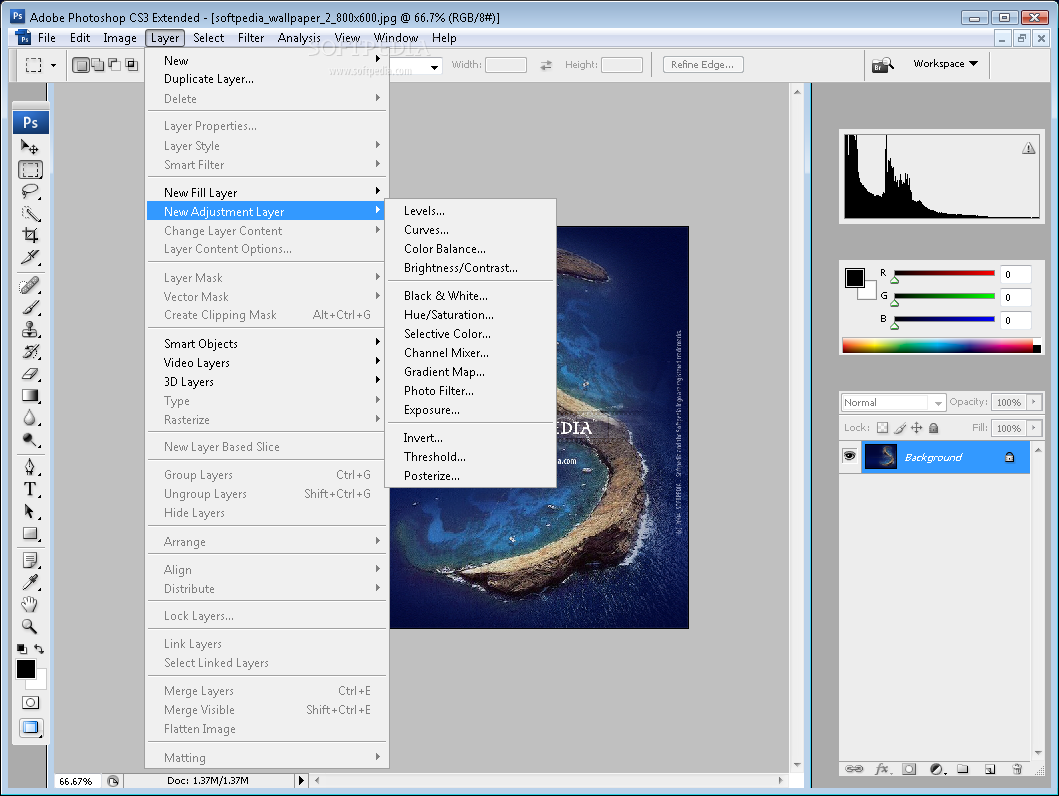
\includegraphics[height=70mm]{data/photoshop.png}
\caption{Captura del programa propietari \emph{Photoshop CS3}.}
\label{photoshop}
\end{figure}

\begin{figure}[ht!]
\centering
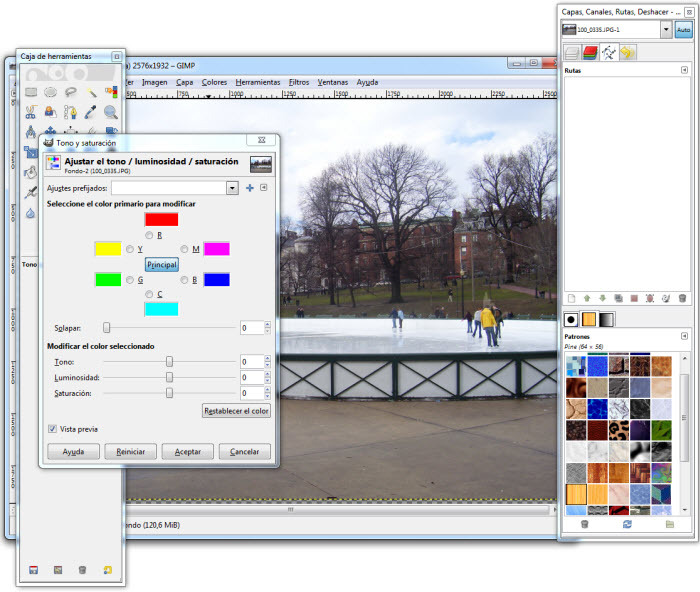
\includegraphics[height=70mm]{data/gimp.jpg}
\caption{Captura de l'alternativa lliure de Photoshop, \emph{GIMP} (GNU Image Manipulation Program).}
\label{gimp}
\end{figure}



\chapter{Llicències de Software}
\section{Definicions}
Abans de parlar sobre els tipus de llicencies software s'haurien 
de conèixer alguns conceptes bàsics.

\begin {itemize}
	\item \emph{Llicencies de software}: són un contracte entre el desenvolupador 
	del software (sotmès a propietat intel·lectual i els drets d'autor), i l'usuari. 
	En aquest contracte es defineixen els drets i deures de ambdues parts. El 
	desenvolupador, o qui hagi cedit els drets d'explotació del producte, és 
	la persona qui decideix quina llicencia software usar per la distribució del 
	programa.
	\item \emph{Patent}: és el conjunt de drets exclusius concedits per un estat al 
	creador o als creadors de un producte susceptible a ser explotat industrialment, 
	per un període limitat de temps a canvi de la divulgació de la invenció. Implica,
	bàsicament, que tercers no poden fer ús de la tecnologia patentada. \cite {definicions}
	\item \emph{Drets d'autor o \textit{copyright}}: és un conjunt de drets i normes \cite {copyright}
	que tenen els autors de creacions de obres de qualsevol tipus, tant científica, 
	tecnològica, didàctica, etc.
\end {itemize}

\section{Tipus de llicencies software}
Hi han molts tipus de llicencies software, però les més utilitzades són aquestes quatre:

\begin{itemize}
	\item \emph{GPL}: prové de \emph{GNU Public License} (GNU essent acrònim de
	\emph{GNU no és Unix}). Aquesta 
	llicència permet la copia, la distribució, tant amb finalitats comercial com no, i 
	la modificació del codi només si es segueix utilitzant el mateix 
	tipus de llicencia, la GPL. No permet la distribució d'executables sense mostrar 
	el codi font d'aquest. És la més usada en el món del 
	software lliure, i garanteix a l'usuari final la llibertat de usar, estudiar, compartir 
	i modificar el software amb el propòsit d'evitar que el software tingui una 
	llicencia de software privativa i protegir-lo dels intents d'apropiació que 
	restringeixin les llibertats de l'usuari.
	
	Si tú utilitzes llibreries amb codi llicenciat GPL, o les modifiques, també has de compartir el teu codi i/o modificacions amb la llicència GPL.
	
	Aquesta llicencia va ser creada per
	\emph{Richard Stallman}, fundador de la \emph{Free Software Foundation}
	pel projecte del grup \emph{GNU}.
	Segons aquest grup, quan es parla de que és \textit{free} es refereixen a que és 
	lliure, no gratuït. \cite {gnugpl} \cite {tldr}
	\item \emph{BSD}: o \emph{Berkeley Software Distribution} és una llicencia software més 
	permissiva que GPL, ja que aquesta té menys restriccions en comparació a la 
	anterior. La llicència BSD, al contrari 
	que la GPL permet l'ús del codi font en software no lliure. Es podria definir com a \emph{llicència molt liberal}. Molts sistemes operatius descendents de BSD són \emph{SunOS, 
	FreeBSD i MacOS X}, entre altres. \cite {bsd} \cite {tldr}
	\item \emph{MIT}: La llicència MIT (Massachusetts Institute of Technology)
	té unes característiques molt similars a la llicència BSD:
	pots fer el que vulguis amb el teu software mentre tu adjuntis el copyright 
	inicial. Hi ha molt software que utilitza la llicència MIT, ja que és simple d'entendre i curta; projecte \emph{Mono}, o \emph{Ruby on Rails}, entre moltes altres.\cite {mit} \cite {tldr}
	\item \emph{WTFPL}: és la llicència més permissiva. Bàsicament, et permet fer
	el que vulguis amb el teu programa com el mateix nom de la llicència indica:
	\emph{Do What The Fuck You Want To The Public Licence}.
	L'usuari pot fer el que vulgui amb el codi font i la llicència en sí, sense
	cap mena de restricció. Aquesta llicència és poc utilitzada, degut a la seva
	falta de restriccions, i el fet que no assegura la continuïtat de les llibertats
	que ella mateixa proporciona.\cite {tldr}
	\item \emph{MPL}: la \emph{Mozilla Public License} és una llicència no lucrativa i poc estricta, que només té uns requeriments molt senzills.
	Els programes que utilitzen aquesta llicència són bàsicament els de la \emph{Mozilla Foundation},
	per exemple el navegador \emph{Firefox} o el client de correus \emph{Thunderbird},
	però també és usat per altres programes, com per la companyia \emph{Adobe} en
	la seva línia de productes \emph{Flex}, o per \emph{LibreOffice}, popular suite
	d'ofimàtica. \cite {tldr}
	
	\item \emph{Sense llicència}: quan un programa no especifica una llicència, l'usuari només té dret a \emph{observar} el codi font d'aquest. Es reserven tots els drets a l'autor, que pot fer el que vulgui amb el programa.
\end{itemize}

\begin{figure}[ht!]
\centering
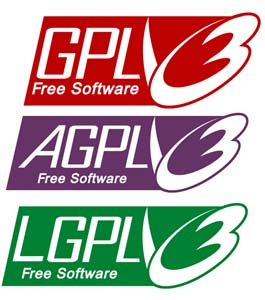
\includegraphics[width=45mm]{data/gpls.jpg}
\caption{Logotips de les diferents versions de la llicència \emph{GNU GPL}.}
\label{gpls}
\end{figure}

\section{Decidir la llicència}
Quan el desenvolupador (o companyia) ha de decidir quin tipus de llicència vol
usar per el seu software ha de tenir en compte les seves motivacions: si aquest
vol remuneració monetària, usarà una llicència de software privativa, la qual estipularà que el seu producte no pot ser compartit ni modificat, o si vol que el seu producte estigui l'abast de 
la comunitat, en aquest cas haurà de decidir el grau de llibertat que vol que tingui 
l'usuari.

De totes formes, cal mencionar la possibilitat de obtenir remuneració econòmica amb llicències
de software lliures: ja sigui a partir de donacions (el mètode més habitual), o amb la
venda directa de l'executable.


\chapter{Moviments de Software Lliure}
\section{Organitzacions defensores del Programari Lliure}

Les organitzacions més influents que s'encarreguen de defensar el software lliure són:
 
 \begin{itemize}
\item \emph{Electronic Frontier Foundation}:  organització sense ànim de lucre basada en part en la primera esmena de la Constitució dels Estats Units, que defensa la llibertat d'expressió, adaptant-la als \emph{ciber-drets}, o \emph{drets virtuals}. Formada en 1990 per \textit{Mitch Kapor, John Gilmore i John Perry}, com a organització lliure vol educar a la premsa, els legisladors i el públic sobre les qüestions de llibertats civils relacionades amb les tecnologies, i actuar per a defensar-les. \cite{OrgDefEFF}
 \cite{OrgDefEFFII}
\item \emph{Free Software Foundation}: Al igual que la \emph{EFF}, és una 		organització sense ànim de lucre fundada per \emph{Richard Matthew Stallman}. És, possiblement, la organització més 		influent de programari lliure, formada alhora per una comunitat ètica en tot el món dedicada 		exclusivament al software lliure i la protecció d'aquest, dividit en diverses etapes:


	\begin{itemize}
	\item Mantenir una definició universal de programari lliure.
	\item Mantenir una educació legal sobre el FOSS, celebrant sovint se- minaris sobre aspectes legals de l'ús de la 		llicència \emph{GPL} (i derivats) i oferint un servei de consulta per a advocats.
	\item Aconseguir que tothom tingui la possibilitat de \emph{tindre control sobre la tecnologia} 	quotidiana, sense restriccions de caire governamental o corporatiu. A través del desenvolupament d'un sistema operatiu completament lliure, es vol aconseguir aquest objectiu. \cite{ObjGNU} \cite{OrgDefFSF}
	\end{itemize}

\end{itemize}

\section{Casos d'èxit de Software Lliure}

\begin{itemize}

\item \emph{GNU}: va ser creat per \emph{Richard Matthew Stallman} el 1983, com a un sistema operatiu (kernel \footnote{Programa que es comunica amb els components d'un ordinador i executa i administra els recursos del mateix.} + utilitats) que es va posar en marxa per a les persones que treballaven i segueixen treballant juntes per la llibertat de tots els usuaris del programari per poder gaudir de tots els graus de llibertat d'una manera \emph{total}. Les motivacions principals que van portar a Richard a dur a terme GNU estan recollides en un document escrit per ell anomenat \emph{GNU Manifesto}. \cite{GNUExit} \cite{GNUExitII} \cite{GnuMan} \cite{GvsM}

\item \emph{Mozilla Corporation}: empresa filial propietària total de la \emph{Fundació Mozilla}, sense ànim de lucre, coordinadora i responsable de la integració d'aplicacions informàtiques tals com el conegut navegador web \emph{Mozilla Firefox} o el client de correu electrònic \emph{Mozilla Thunderbird} en el món informàtic. Aquests programes s'actualitzen diàriament per mitja de milers de programadors voluntaris que treballen juntament amb els de la corporació que es regeixen per uns principis que l'empresa té establerts. \cite{MozExit} \cite{MozExitII} \cite{MozFesto}

\item \emph{GNU/Linux}: és un sistema operatiu lliure, format pel \emph{kernel} Linux i les utilitats del projecte GNU. Dissenyat per milers de programadors d'arreu del món, segueix en desenvolupament sota la coordinació de \emph{Linus Torvalds}. Cada dia s'actualitzen nous continguts, que milloren el funcionament del sistema operatiu. \cite{LinExit} \cite{POSIX}

\item \emph{Chromium}: és un projecte de navegador de codi obert que té com a objectiu construir una manera més segura, més ràpida i estable per als usuaris d'experimentar amb internet. El navegador conté documents de disseny, informació de proves i altres continguts per ajudar a aprendre, construir i treballar amb el seu codi font. També es la base de \emph{Google Chrome}, la versió propietària desenvolupada per \emph{Google}. \cite{Chrom} 
\end{itemize}

\begin{figure}[ht!]
\centering
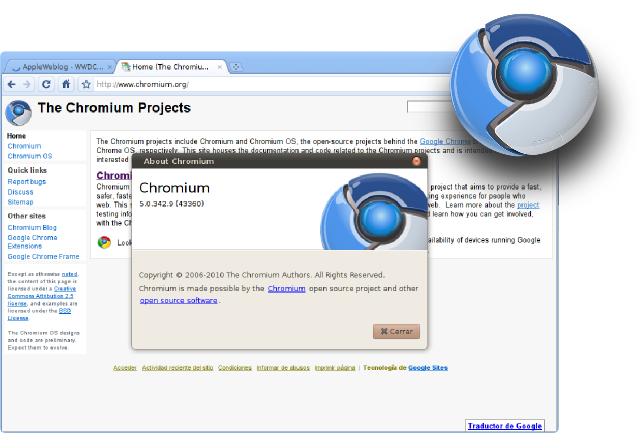
\includegraphics[width=36mm]{data/chromium.png}
\caption{Imatge del navegador lliure Chromium.}
\label{chromium}
\end{figure}


\chapter{Intel·ligència Artificial}
\section{Què és?}

La intel·ligència artificial és aquella branca de la informàtica dedicada al
desenvolupament d'algorismes per a conseguir que una màquina prengui decissions
 racionals per si mateixa o que es comporti de forma similar a la intel·ligència humana.

En resumides comptes, segons la definició més estesa, que és la de l'informàtic i
investigador cognitiu estadunidenc \emph{John McCarthy}, és \emph{"Fer que una màquina
es comporti d'una manera que en un humà considerariem intel·ligent"}.

En el que a robòtica es refereix la intel·ligència artificial consisteix a aplicar la
definició anterior, és a dir, un ésser no viu amb una intel·ligència racional semblant
a la humana, a una estructura que sol tenir una fisiologia semblant a la nostre i que
es pot moure.
\cite{definiciondeia} \cite{wikiia} \cite{monoia}

\section{Principals utilitats}

És interessant veure a on s'utilitzen mètodes d'IA en l'actualitat. És també complicat fer-ho sense reflexionar una mica, ja que la convicció popular de IA és relacionada amb la simulació del caràcter humà, i si més no estem encara una mica lluny d'aquest objectiu, hi ha una gran quantitat d'aplicacions que utilitzen petits procediments de forma similar a com ho faria un humà.

La IA s'utilitza diàriament en àmbits extremadament diversos: diagnosi mèdica \ref{diagnosis}, comerç amb stock, control de robots, llei, traducció de textos \ref{translate}, domòtica, visió artificial \ref{cat}, etc.


\begin{figure}[ht!]
\centering
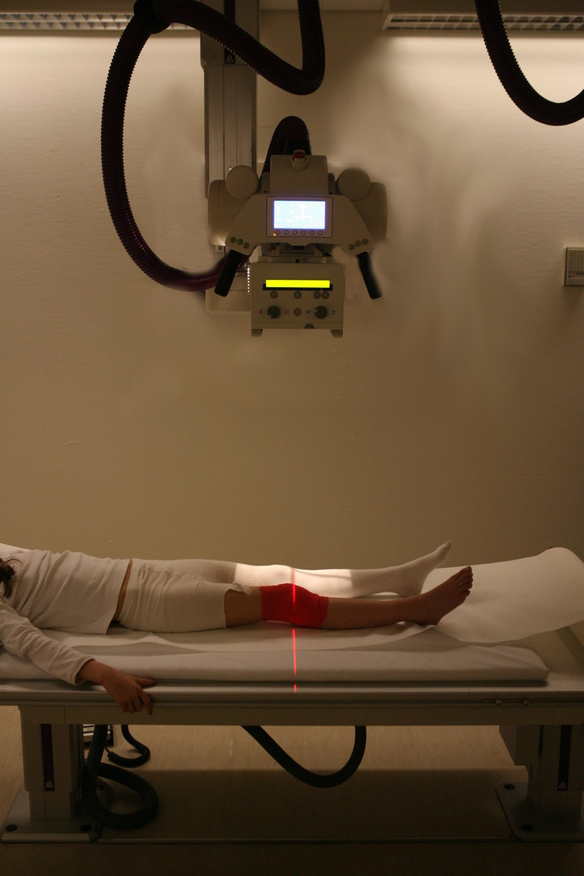
\includegraphics[height=60mm]{data/diagnosis_2.jpg}
\caption{S'estan dissenyant sistemes de \emph{diagnosi mèdica}, que seran entrenats per a, per exemple, distingir teixits cancerígens en imatges.}
\label{diagnosis}

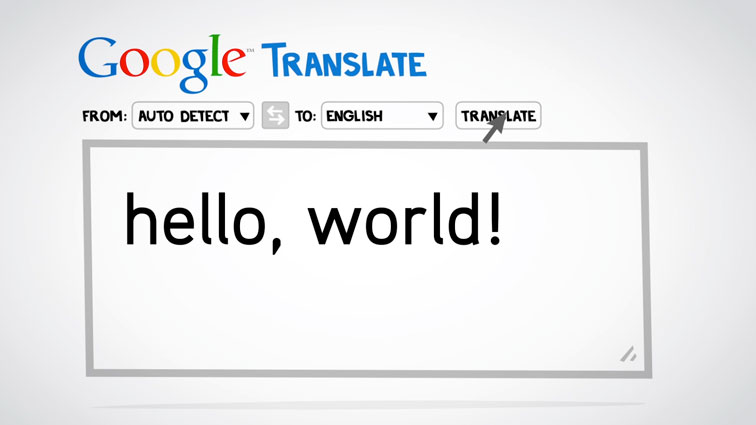
\includegraphics[width=60mm]{data/translate.jpg}
\caption{S'utilitza de forma diària, però molts pocs saben que darrere d'una interfície d'usuari senzilla s'amaga un sistema de traducció intel·ligent molt diferent a la traducció literal paraula per paraula.}
\label{translate}

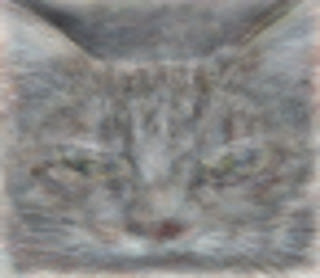
\includegraphics[width=75mm]{data/cat.jpeg}
\caption{Desenvolupadors de Google han entrenat una \emph{xarxa neuronal} per a que identifiqui cares de gats en vídeos a YouTube. Aquesta es la visió generalitzada d'un gat, després de milers de vídeos d'entrenament. \cite{googlecat}}
\label{cat}
\end{figure}

\chapter{Present i futur IA}
\section {Present de la IA}
Actualment, el camp de la IA s'ha especialitzat molt: \emph{aprenentatge de màquina}, \emph{robòtica aplicada}, \emph{deducció, raonament i solució de problemes}, \emph{processament de llenguatge natural}, \emph{moció i manipulació}, \emph{percepció}, \emph{intel·ligència social}, \emph{creativitat}, i l'objectiu final: \emph{intel·ligència artificial general}, que combina tots els aspectes.

En el nostre dia a dia i han molts programes que utilitzen intel·ligència artificial (de forma més o menys proficient) sense que ens n'adonem, com per exemple, el \emph{traductor de Google}: sembla molt fàcil buscar al diccionari les paraules que es demanen per a traduir, però una traducció literal mai és satisfactòria, per això es segueixen procediments intel·ligents que permeten realitzar traduccions naturals.

\emph{YouTube} i \emph{Google} utilitzen algorismes intel·ligents per a filtrar resultats de cerca segons els teus gustos. \emph{eBay} i \emph{Amazon} també ho fan, recomanant productes d'acord amb el teu historial de compra.


Pel que fa l'àmbit de la robòtica, s'han creat robots capaços de caminar de forma òptima i evitar caigudes causades per els diferents tipus de terreny intentant simular animals com
ara gossos en córrer. També s'han creat humanoides, robots amb forma de persones, que són capaços de fer moviments humans, per exemple abraçar expressar emocions i manipular certs objectes. \cite{bostondynamics}


Un altre exemple d'intel·ligència artificial és la que s'utilitza per complementar (o formar) un programa informàtic; el reconeixement per veu es un bon exemple. \emph{Apple} utilitza la interpretació de la veu humana per a crear una aplicació que respon a qualsevol pregunta.

\section {Futur de la IA}
És difícil predir quin serà el futur de la intel·ligència artificial, però podem establir uns objectius per al futur.

Un dels objectius que tenen la majoria de persones que treballen en la IA és aconseguir que aquesta intel·ligència deixi de ser tant especifica i passi a ser global; capaç d'aprendre
qualsevol cosa, analitzar-la de manera intel·ligent i pensar bàsicament com les persones humanes. Aquest objectiu encara és difícil d'aconseguir perquè si volem que pensin com a éssers
humans primer hem de saber perquè pensem com a éssers humans.

Aquest concepte pot semblar estrany però el que pretenem dir és que hem d'entendre primer com funciona el nostre cervell
per raonar, com reacciona en situacions que no coneix i com emmagatzema informació. Per tant podem dir que la IA pot estar lligada a la neurociència i que, en part,
depèn d'ella; el desenvolupament de la neurociència porta de la ma el desenvolupament de la intel·ligència artificial.


Un altre dels objectius de futur de la IA és el que fa referència a la intel·ligència específica, i en aquest cas està més a l'abast dels programadors. Un dels molts projectes de aquesta
intel·ligència és el de cotxes que siguin capaços de conduir sense la necessitat de un conductor. Aquest programa podria evitar molts accidents causats pel consum de drogues o
d'alcohol, i la incapacitat de persones grans al volant, fent més segures les carreteres i evitant errors humans que a qualsevol persona podem passar-li.

%\section {Perillositat de la IA}
%La discussió de si pot arribar a ser perillosa o no una IA capaç %de pensar com un humà dóna molt a parlar i discutir ja que s'han %de tenir en compte molts factors.

%Si en algun moment s'aconsegueix una intel·ligència artificial capaç de pensar com els humans però de una manera més eficient i calculadora, si tingués ment per pensar i raonar podria arribar
%a pensar que nosaltres, els éssers humans, no tenim cap funció ja que faríem el mateix que fan elles però de una manera menys eficient amb més defectes i això la podria fer pensar que hauríem
%de desaparèixer i per tant ella voldria eliminar als seus creadors. No seria perquè ens tingués odi, però tampoc ens tindria amor ni compassió, simplement pensaria que som inservibles i per tant
%ens eliminaria com si nosaltres tiréssim una joguina o un electrodomèstic a la paperera perquè ja l'únic que fa es ocupar-nos espai que podria ser utilitzat per una altre cosa, i pel que fa
%els éssers humans estaríem gastant recursos que podrien ser utilitzats per recerca. Aquesta situació espantosa i clarament alarmant es podria evitar aplicant un dels dos factors més importants
%que fan els ésser humans tal com són: els valors i les emocions. Si ens preguntessin que ens diferencia del animals diríem que clarament és la intel·ligència, que en part és veritat, però el
%factors que ens permet viure en comunitat i diferenciar-nos dels animals són els valors, que ens impedeixen fer accions que estan en contra la nostra moral, i les emocions, que ens permeten
%reaccionar amb l'exterior. Per tant si una màquina té valors i emocions i nosaltres la tractem com un igual no tindria el pensament de eliminar-nos i podria viure ajudant-nos màquines i humans.

\section {Velocitat d'evolució}
Es podria dir que hem avançat molt en el camp de la intel·ligència artificial en els últims anys, però tenim problemes per a continuar evolucionant. Això és
donat per diversos factors \cite{pbs}:
\begin {itemize}
\item \emph{Neurociència:} com hem explicat en un dels apartats anteriors, encara es té un desconeixement molt gran sobre el funcionament del cervell; això impedeix simular-lo, evidentment.
\item \emph{Desconeixent general:} hi ha un clar desconeixement general de la intel·ligència artificial, degut a que es tracta d'un camp en continuu desenvolupament, amb molts poques \emph{lleis} que es segueixen al peu de la lletra en qualsevol cas, i molts models matemàtics que materialitzar.
\item \emph{Falta d'inversió:} els governs d'avui en dia no consideren un factor important la intel·ligència artificial i aquest factor va lligat amb el factor anterior: el desconeixement.
\item \emph{Poder computacional:} si en una cosa coincideixen molts científics, es en que el cervell és una màquina de càlcul molt potent, que realitza interconnexions de forma molt ràpida, continua, i paral·lela. Els ordinadors han d'avançar en poder computacional per a poder establir-se al nivell del cervell humà, o s'han d'optimitzar els algorismes. Tot i la increïble potència dels processadors actuals (\emph{1,16 bilions} de transistors en un de quatre nuclis), s'estima que el cervell té \emph{100 bilions} de neurones. A més a més, un transistor no es tradueix a una neurona, la qual cosa implica multiplicar el nombre final per arribar a una quantitat de transistors realista.
\end {itemize}

\begin{figure}[ht!]
\centering
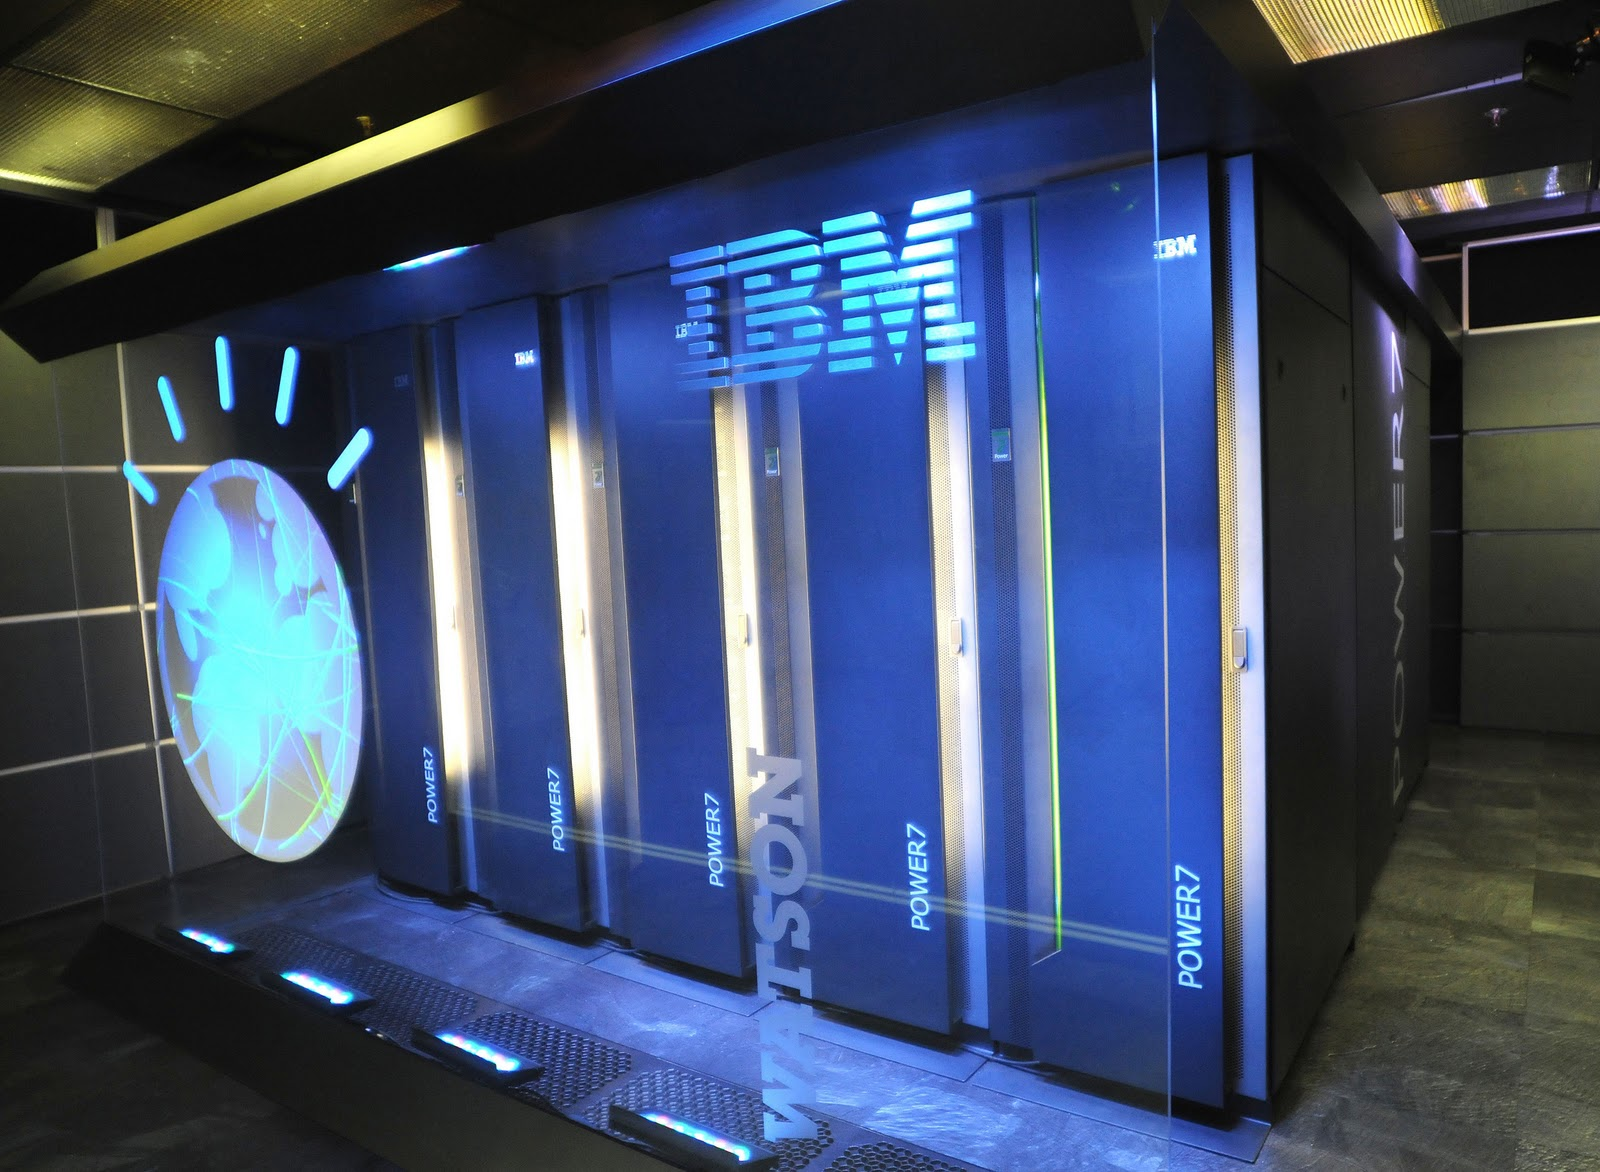
\includegraphics[height=75mm]{data/watson.jpg}
\caption{El \emph{super-ordinador} d'IBM, \emph{Watson}, posseeix 16,000 gigabytes de memòria RAM (comparats amb els 4 d'un ordinador corrent), 90 processadors de 8 nuclis cadascun (720 nuclis en total, comparats amb els 2 d'un ordinador corrent), i 4,000 gigabytes de disc dur (comparats amb els 500 d'un ordinador corrent) \cite{watsonspecs}. Va guanyar als dos millors oponents del programa nord-americà \emph{Jeopardy!} \cite{watsonjeopardy}.}
\label{watson}
\end{figure}


\chapter{La historia de la IA}
\section{Introducció}

El concepte d'una \emph{màquina pensant} es va introduir el 2500 a.C, quan els egipcis buscaven en estàtues parlants consells místics. Segles després, durant el segle XV, els autòmats preferits de al societat eren els ossos que tocaven tambors i figuretes ballarines que apareixien cada vegada que un rellotge marcava l'hora. \emph{Isaac Asimov}, un símbol en el camp de la robòtica, va ser escriptor, erudit i autor de les lleis de la mateixa. \emph{Asimov} estaba anys llum dels pensadors de l'època i va fer prediccions en les quals la \emph{cibernètica} (a Asimov li agradava referir-se a la robòtica amb el nom de cibernètica), provocaria una revolució intel·lectual. 
Issac Asimov va escriure en el pròleg de \emph{Thinking by Machine: a Study of Cybernetics}, de \emph{Pierre de Latil}:

\begin{quote}
\emph{``La cibernètica no és merament una branca de la ciència, és una revolució intel·lectual que rivalitza en importància la Revolució Industrial. És possible que al igual que una màquina pot fer-se càrrec de les funcions rutinàries dels músculs humans, un altre pugui fer-se càrrec dels usos de rutinaris de la ment humana?''}

\end{quote}

Finalment el terme va ser establert el 1956, en la \emph{Conferència de Darmouth}, un congrés en el qual es van fer previsions triomfalistes a deu anys que mai es van complir, el que va provocar l'abandó gairebé total de les investigacions durant quinze anys. En la \emph{Conferencia de Darmouth} es va intentar esbrinar com fabricar màquines que, utilitzant el llenguatge natural, formessin abstraccions i conceptes, i siguessin capaces d'auto-millorar-se; l'estudi va durar 2 mesos i estava format per 10 persones. El matemàtic, lògic, científic de la computació, criptògraf  i filòsof britànic \emph{Alan Turing} ja havia dissenyat en el 1936-1937 la \emph{Maquina de Turing} (model computacional que va demostrar que no hi ha un mètode definit que es pugui aplicar a qualsevol sentència matemàtica). La pregunta bàsica que Turing va tractar de respondre era \cite{Matur} \cite{Algor}: 

\begin{quote}
	\emph{``Poden les maquines pensar?''}
\end{quote}

Els arguments a favor de Turing sobre la intel·ligència artificial, van iniciar un debat intens que va marcar clarament la primera etapa d'interacció entre la intel·ligència artificial i la psicologia. De fet, se sap que anys enrere diferents filòsofs i matemàtics ja pensaven tant en la intel·ligència artificial com en el seu funcionament; per exemple, Aristòtil, va ser el primer en descriure de manera estructurada un conjunt de regles que descrivien el funcionament de la ment humana \cite{IAgen} \cite{IAgenII}.

\section{Evolució de la IA}

\begin{figure}[ht!]
\centering
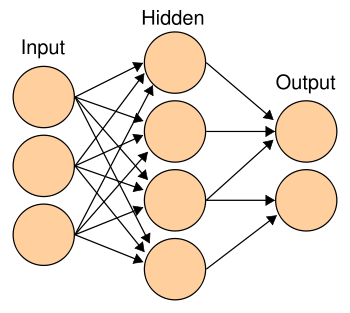
\includegraphics[height=35mm]{data/nn.png}
\caption{Esquema simple d'una xarxa neuronal de topologia 3-4-2.}
\label{nn}
\end{figure} 


\begin{itemize}
\item  \emph{Aristòtil} (300 a.C): va ser el primer en descriure de manera estructurada un conjunt de regles que descrivien el funcionament de la ment humana
\item  \emph{Ctesibi d'Alexandria} (250 a.C): va desenvolupar una màquina capaç de regular el flux d'aigua que actua modificant el comportament de la màquina.
\item \emph{Gottlob Frege} (1879): amplià la lògica booleana i establí la \emph{Lògica del Primer Ordre} (sistema lògic-deductiu que restringeix quines són les expressions correctament formades). Aquesta ordre és tant summament important que té el poder expressiu suficient per definir pràcticament totes les matemàtiques.
\item \emph{Lee De Forest} (1903): inventa el tríode, un component electrònic usat per amplificar, commutar, o modificar una senyal elèctrica. \cite{Tri}
\item \emph{Alan Turing} (1936-1937): considerat com el pare de la ciència informàtica, va formular el concepte de \emph{algorisme}, i va inventar la \emph{Màquina de Turing}. Va ajudar a Anglaterra contra els Alemanys en la Segona Guerra Mundial i va publicar un article on es va demostrar que existeixen problemes dels quals no es pot obtenir una solució; ni per mitjà humà ni per l'ús de computadores.
\item \emph{Warren McCulloch i Walter Pitts} (1943): van formular un model de \emph{neurones artificials} \ref{nn} sense considerar-se un treball del camp de la intel·ligència artificial degut a la inexistència d'aquesta en la època.\cite{EvoIA}
\item \emph{Introducció de la lògica} (1958): en John McCarthy va introduir la lògica en la recerca de la IA, i el 1963, en J. Alan Robinson havia descobert un simple mètode per a implementar la deducció en programes informàtics \cite{machineswhothink}.
\item \emph{Backpropagation} (1982): Rumelhart, Hinton i Williams popularitzen el nou mètode per a entrenar xarxes neuronals \cite{mlintro}, la \emph{propagació marxa enrere}, que s'utilitza avui en dia en molts dels dissenys de xarxes neuronals \cite{mlalgo09}.
\item \emph{Cyc} (1984): s'inicia una base de dades que pretén emmagatzemar els coneixements que tot ésser humà en una cultura moderna té. El projecte es manté actiu avui dia, amb una alternativa lliure, \emph{OpenCyc} \cite{opencyc}.
\item \emph{Deep Blue} (1997): super-ordinador que va guanyar al campió d'escacs Garry Kasparov \cite{deepblue}.
\item \emph{Watson} (2011): super-ordinador que va guanyar als dos millors participants del programa nord-americà \emph{Jeopardy!} \cite{watsonjeopardy}.
\end{itemize}

\section{El test de Turing}

\emph{Alan Turing}, va dissenyar un simple i lògic model matemàtic durant 1950 capaç de \emph{verificar si una màquina és o no intel·ligent}.

El test és duu a terme simplement situant un humà i una màquina separats per una paret. El test es basarà en l'humà, que haurà de anar formulant preguntes i la màquina les haurà de respondre. L'humà, al ser inconscient de que està parlant amb una màquina, haurà de jutjar si les respostes que rep són lògiques, o no. Si creu que ho són, es considerarà que la màquina en qüestió és intel·ligent. \cite{Matur}


\bibliographystyle{plain}
\bibliography{biblios/biblio,biblios/biblio_gonzalo,biblios/soft_propietari,biblios/soft_lliure,biblios/software_lliure}

\end{document}
